\section{Results}
\label{sec:results}

In this section the main results of this work are presented, namely the
determination of the photon PDF $x\gamma(x,Q)$ from a fit to 
HERA inclusive structure functions and ATLAS high-mass Drell-Yan cross sections.
%
First of all, the resulting photon PDF is shown and compared with other
recent extractions.
%
The impact of the high mass DY data on
the quark and gluon PDFs is also quantified.
%
Then the robustness of the results to varying the model, parametrization, and procedural
inputs that affect our fit of $\gamma(x,Q)$ is assessed.
%
Finally, perturbative stability is addressed by comparing NLO and
NNLO results.

\subsection{Comparison between experimental data and fit results}

In the following, the results that will be shown
correspond to those obtained from fitting the
double-differential $\lp m_{ll},y_{ll}\rp$ distributions.
%
We have verified that comparable results are obtained if the
$\lp m_{ll},\Delta\eta_{ll}\rp$ distributions are fitted instead.
%
Using the NNLO fit settings discussed in Sect.~\ref{sec:fitsettings},
a $\chi^{2}/N_{\rm dof} = 1235.85/1056$ is obtained, with a partial
$\chi^2/N_{\rm data} = 47.96/48$ for the high-mass Drell-Yan data,
where $N_{\rm dof}$ is the number of degree of freedom in the fit and 
$N_{\rm data}$  is the number of data points for high-mass DY data.

Figs.~\ref{hmDY_2D_1}--\ref{hmDY_2D_3} show the comparison between the ATLAS
high-mass Drell Yan data and the NNLO predictions for all the mass
bins of the $(y_{ll},m_{ll})$ distribution.
%
The fit results are denoted as {\tt xFitter\_epHMDY}.
%
In the lower panel the ratio of theory over data is shown, where the
yellow band corresponds to the correlated systematic uncertainties.
%
The band around the theory prediction corresponds to the total theory
uncertainty from the PDF fit. 
%
The shifts due to systematic uncertainties are indicated by a dashed
line.


%%%%%%%%%%%%%%%%%%%%%%%%%%%%%%
\begin{figure}[t]
\centering
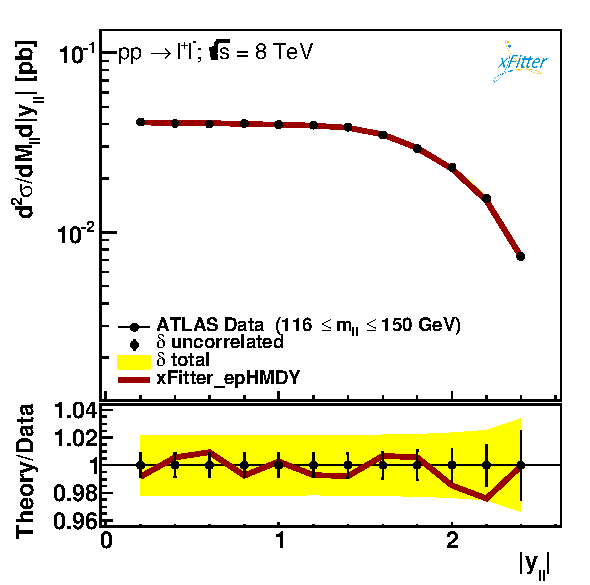
\includegraphics[width=14cm]{figs/data_401-1.pdf}\\
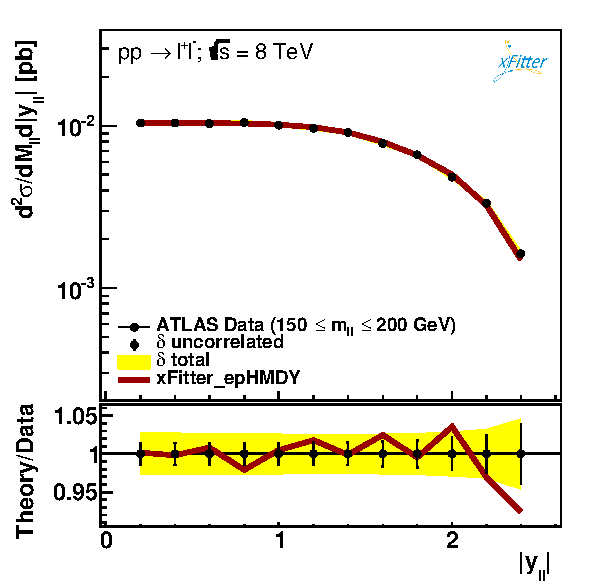
\includegraphics[width=14cm]{figs/data_402-1.pdf}
\caption{Comparison between the results of the fit and the ATLAS data
  for the $(m_{ll},|y_{ll}|)$ double-differential Drell-Yan cross-sections
  as function of $|y_{ll}|$, for the first two $m_{ll}$ bins.
  %
  The comparisons are shown both
  in an absolute scale (left plots) and as ratios to the central value
  of the experimental data (right plots).
  %
  The error bars on the data points correspond to the statistical
  uncertainties, while the yellow bands
  indicate instead to size of the correlated systematic uncertainties.
  %
  The solid lines indicate the theory calculations obtained using the results
  of the fit {\tt xFitter\_epHMDY}, with the dashed lines including as well the systematic shifts.
  %
  In the lower panels of ratio plots, we show the $\chi^2$ pulls between fit and data for each $y_{ll}$
  bin.
}
\label{hmDY_2D_1}
\end{figure}

%%%%%%%%%%%%%%%%%%%%%%%%%%%%%%
\begin{figure}[t]
\centering
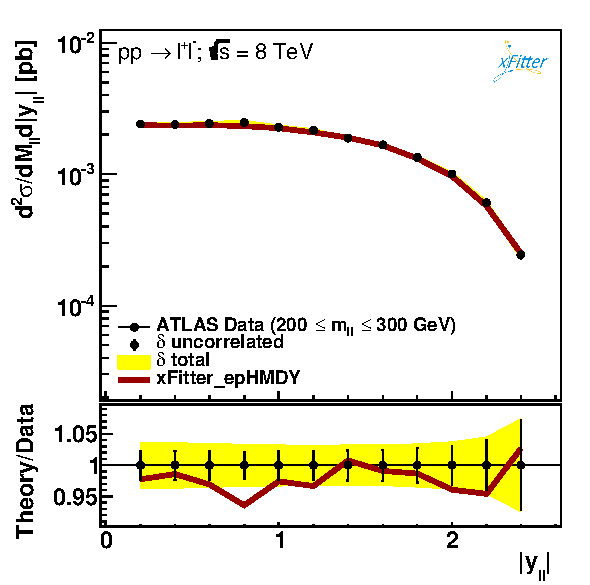
\includegraphics[width=14cm]{figs/data_403-1.pdf}\\
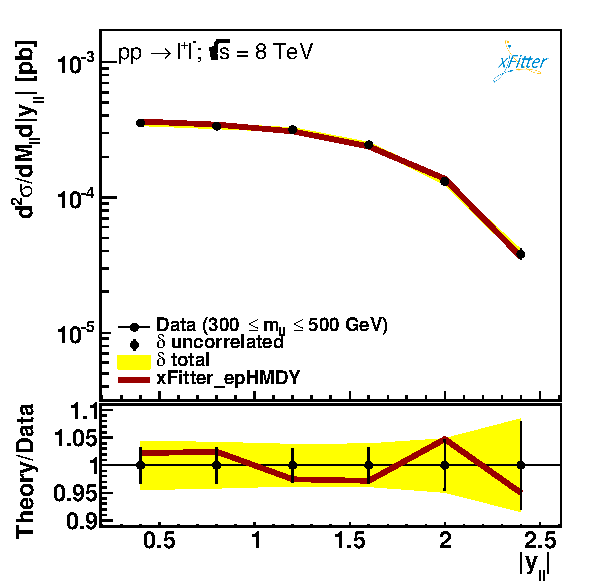
\includegraphics[width=14cm]{figs/data_404-1.pdf}
\caption{Same as Fig.~\ref{hmDY_2D_1} for the third and fourth $m_{ll}$ bins.
}
\label{hmDY_2D_2}
\end{figure}

%%%%%%%%%%%%%%%%%%%%%%%%%%%%%%
\begin{figure}[t]
\centering
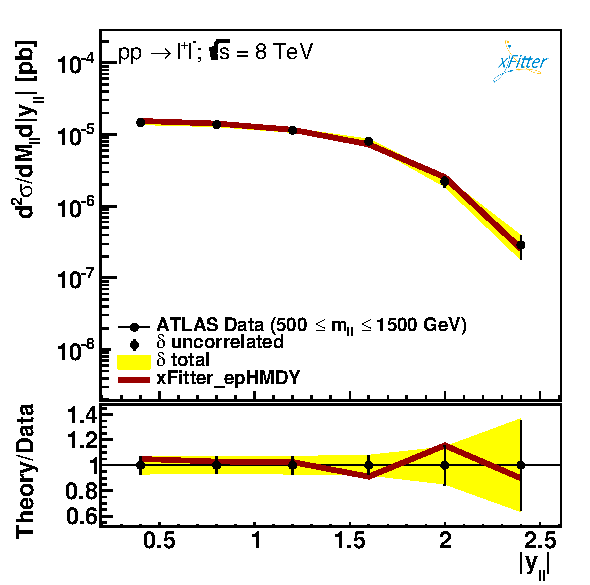
\includegraphics[width=14cm]{figs/data_405-1.pdf}
\caption{Same as Fig.~\ref{hmDY_2D_1} for the highest $m_{ll}$ bins.
}
\label{hmDY_2D_3}
\end{figure}
%%%%%%%%%%%%%%%%%%%%%%%%%%%%%%%

As can be seen from Fig.~\ref{hmDY_2D_1}--\ref{hmDY_2D_3}, once the shifts due to
experimental systematic uncertainties have been accounted for, there
is a reasonable agreement between ATLAS data and NNLO theory
predictions.
%
This agreement is consistent with the values of the $\chi^2$ reported in
Table~\ref{tab:chi2fit}. The agreement is particularly impressive even 
the high precision of this measurement with experimental
errors at the few percent level in most of the kinematic range
available.


\subsection{The photon PDF from high-mass DY data}
%
The results for the photon PDF and the impact
of the DY measurements on the quark and gluon PDFs are presented.
%

In Fig.~\ref{photon_zoom} the $x\gamma(x,Q)$ distribution at
$Q^2=10^4$ GeV$^2$ with experimental uncertainty band using MC method is presented and compared to LUXqed~\cite{Manohar:2016nzj},
HKR~\cite{Harland-Lang:2016apc} and NNPDF3.0QED sets.
%
For NNPDF3.0QED, we show the 68\% CL uncertainty, while for LUXqed the
uncertainty band is obtained by adding in quadrature all the model
variations.

%%%%%%%%%%%%%%%%%%%%%%%%%%%%%%%%%%%%%%%%%%%%%%%%%%%%%%%%
\begin{figure}[t]
  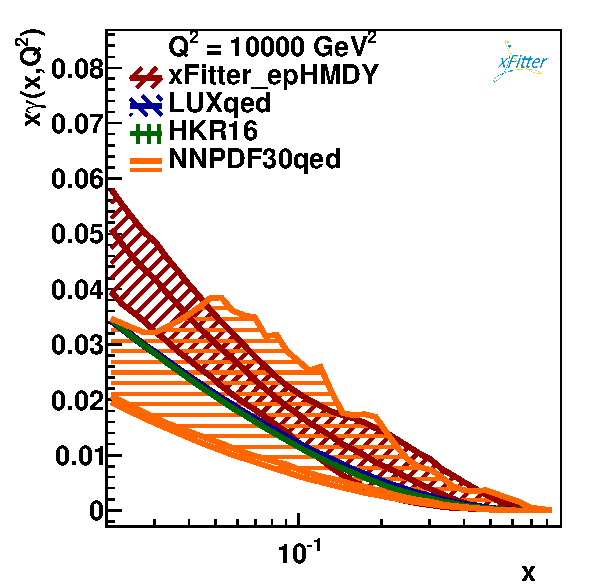
\includegraphics[width=8cm]{figs/photon_comp_10000.pdf}
  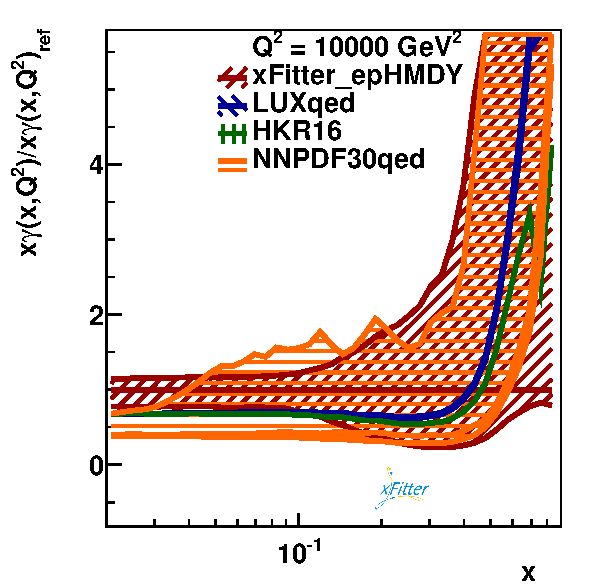
\includegraphics[width=8cm]{figs/photon_comp_10000_ratio.pdf} 
\caption{Left: comparison between $x\gamma(x,Q^2)$ at $Q^2=10^4$ GeV$^2$ in the present
  NNLO analysis with the corresponding results from NNPDF3.0QED, LUXqed and HKR16.
  %
  Right: the same comparison now with the results normalized to the central value
  of {\tt xFitter\_epHMDY}.
  %
  For HKR16, only the central value is shown, while LUXqed includes
  the associated uncertainty band obtained following the prescription
  of~\cite{Manohar:2016nzj} }
\label{photon_zoom} \label{photon_zoom_ratio}
\end{figure}
%%%%%%%%%%%%%%%%%%%%%%%%%%%%%%%%%%%%%%%%%%%%%%%%%%%%%%%%

Fig.~\ref{photon_zoom} shows that in the region
where the HMDY predictions are sensitive to the photon PDF, there is
good agreement between the four determinations.
%
The PDF uncertainties in the current
analysis are reduced compared to those of NNPDF3.0QED, though they are still not competitive with those
of LUXqed.
%
There is excellent agreement between the LUXqed and the HKR
calculations, illustrating the commonalities between the two
approaches.
%
Fig.~\ref{photon_zoom_ratio} shows the same comparison of
different results for the photon PDF $x\gamma(x,Q)$ now normalized to
the central value of {\tt xFitter\_epHMDY}.
%
This format allows the relative compatibility
between the various results to be assessed, as well as the relative size of the PDF
uncertainties.
%
The experimental uncertainty on {\tt xFitter\_epHMDY}
is at the $\sim 30\%$ level, depending on the specific value of $x$,
improving over NNPDF3.0QED but still far from the percent accuracy of
the LUXqed calculation.

The impact of the high-mass Drell-Yan 8 TeV measurements on
the light quark PDFs can also be assessed.
%
For this purpose, and since HERA data alone (which should be used as
benchmark for this comparison) does not have sensitivity on the photon
PDF, the fits have been repeated freezing the photon PDF to the
shape given by HMDY data, such that
a meaningful comparison between the HERA-only
baseline and the HERA+HMDY fit can be performed, to gauge the modifications of quark and
gluon PDFs.
%
This comparison is shown in Fig.~\ref{fig:QCDfit} for the up and down
antiquarks, for which the effect of the high-mass Drell-Yan data is
expected to be most pronounced. PDFs are presented as ratios to the
central value of the HERA+HMDY fit with their experimental uncertainties.
%
As is apparent from this comparison, the modifications in the medium
and large-$x$ antiquark distributions from the HMDY data are
significant for $x\ge 0.01$, although the two fits agree always at the
one-sigma level.
%
The improvement of the PDF
uncertainties is particularly marked for the case of $x\bar{d}$,
%
These results were cross-checked with fits obtained by switching
off the QED effects for both HERA only fits and the nominal fits, with
the same outcome.

%%%%%%%%%%%%%%%%%%%%%%%%%%%%%%
\begin{figure}[t]
\centering
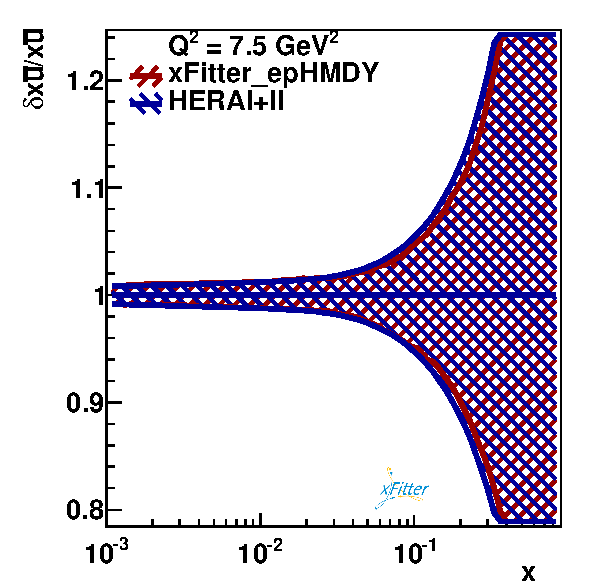
\includegraphics[width=8cm]{figs/q2_7_5_pdf_ubar_ratio.pdf}
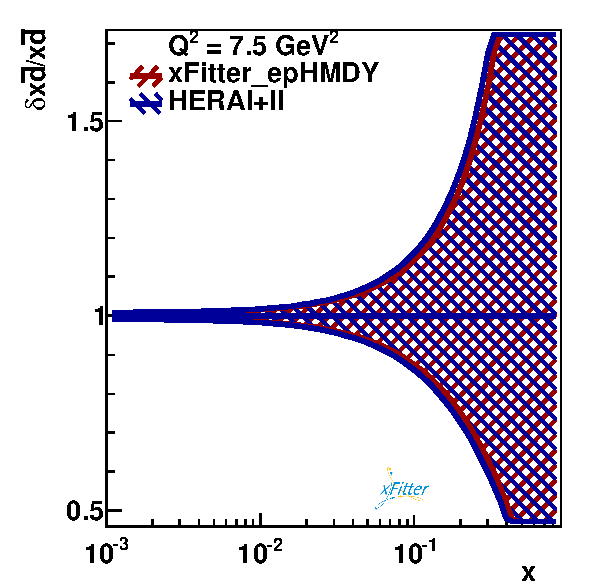
\includegraphics[width=8cm]{figs/q2_7_5_pdf_dbar_ratio.pdf} 
\caption{The impact of the ATLAS high-mass 8 TeV Drell-Yan measurements
  on the $x\bar{u}$ and $x\bar{d}$ sea quark PDFs at the starting scale $Q^2=7.5$ GeV$^2$.
  %
  Results are shown normalized to the central value of the HERA+HMDY
  fit.  }
\label{fig:QCDfit}
\end{figure}
%%%%%%%%%%%%%%%%%%%%%%%%%%%%%%%

After this comparison at the level of PDFs, a quantitative comparison
between theoretical predictions and high-mass Drell-Yan measurements is presented.
%
The values of the $\chi^2$ for the HERA structure functions and for
the high-mass DY data for the NNLO fit are summarised in
Table~\ref{tab:chi2fit}.
%
As can be seen, the agreement between data and NNLO predictions is
very good for all the bins in $m_{ll}$ of the $8$ TeV Drell-Yan data.
%
For the sum of all the five rapidity bins, we find a $\chi^2=48$ for
$48$ data points.
%
The quality of the agreement with the HERA inclusive structure
functions is of comparable quality to that found in the HERAPDF2.0 analysis~\cite{}.
%
In the calculation of the total $\chi^2$, the correlations between the
different $m_{ll}$ bins have been taken into account.

%%%%%%%%%%%%%%%%%%%%%%%%%%%%%%%%%%%%%%%%%%%%
\begin{table}[t]
  \centering
  \begin{tabular}{|c|c|}
    \hline
    Dataset  &   $\chi^2$ \\
    \hline
    \hline
    HERA I+II & 1235.85/1056\\
    \hline
    HMDY  116 GeV $\ge m_{ll} \ge $ 150 GeV  &  8.96/12 \\
    HMDY  150 GeV $\ge m_{ll} \ge $ 200 GeV  &  15.36/12 \\
    HMDY  200 GeV $\ge m_{ll} \ge $ 300 GeV  &  13.81/12 \\
    HMDY  300 GeV $\ge m_{ll} \ge $ 500 GeV  &  4.82/6 \\
    HMDY  500 GeV $\ge m_{ll} \ge $ 1500 GeV &  3.96/6 \\
    \hline
    Correlated (HMDY) $\chi^2$ & 1.17 \\
    Log penalty (HMDY) $\chi^2$  & -0.12 \\
    \hline
    \hline
    Total  (HMDY) & 47.96/48 \\
    \hline
    \end{tabular}
  \caption{$\chi^{2}$ for high-mass Drell Yan data for the NNLO fit.
    %
    The results for the individual $m_{ll}$ bins are shown
    as well as for the total dataset.
\label{tab:chi2fit}
  }
\end{table}
%%%%%%%%%%%%%%%%%%%%%%%%%%%%%%%%%%%


Following this presentation of the main features of the {\tt
  xFitter\_epHMDY} analysis, the stability of the fit and its robustness
to model, parametrization, and procedural uncertainties are assessed.

\subsection{Robustness and perturbative stability checks}
\label{sec:crosschecks}

In this section the robustness of our determination of the
photon PDF $x\gamma(x,Q)$ is assessed with respect to a number of variations.
Firstly variations of the values of
physical parameters, like $\alpha_s$ or the charm mass are explored, secondly
variations of the choices made for the PDF parametrization, and thirdly 
variations associated to different fitting procedures.
%
One variation at a time is explored and its effect on the
central value of the photon PDF is compared with the size of the experimental
uncertainty computed using the Monte-Carlo method.

Firstly, the impact of uncertainties associated to either
the choice of some physical parameters or of some specific settings
adopted in the fit are explored.
%
Fig.~\ref{fig:model} shows the comparison between the baseline
determination of $x\gamma(x,Q)$ at $Q^2=10^4$ GeV$^2$ in the present
analysis (including the experimental uncertainties) with the central
value of those fits for which a number of variations have been
performed.
%
In particular, we have considered the following variations:
\begin{itemize}
\item The strong coupling constant is varied by $\delta \alpha_s=\pm 0.002$ around the central value.
\item The ratio of strangeness to non-strange PDFs is decreased to $r_s=0.75$ instead of $r_s=1$.
\item The value of the charm mass is varied between $m_c=1.41$ GeV and $m_c=1.53$ GeV,
  and that of the bottom mass between $m_b=4.25$ GeV and $m_b=4.75$ GeV.
\item The minimum value $Q_{\rm cut}$ of the fitted data is decreased down to $\sqrt{5}$ GeV.
\item The parametrization scale $Q_0$ is raised to $\sqrt{10}$ GeV as compared
  to the baseline value of $Q_0=\sqrt{7.5}~$GeV.
\end{itemize}
The results of Fig.~\ref{fig:model} show that in all cases the effect
of all the variations is contained within (and typically much smaller than) 
the experimental PDF uncertainty bands of the reference fit.

%%%%%%%%%%%%%%%%%%%%%%%%%%%%%%                                                                                                                                                                           
\begin{figure}[t]
\centering
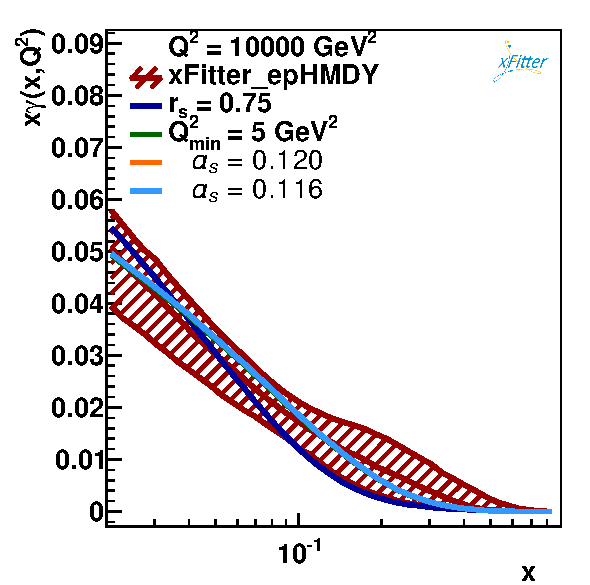
\includegraphics[width=8cm]{figs/q2_10000_pdf_ph_model_1}
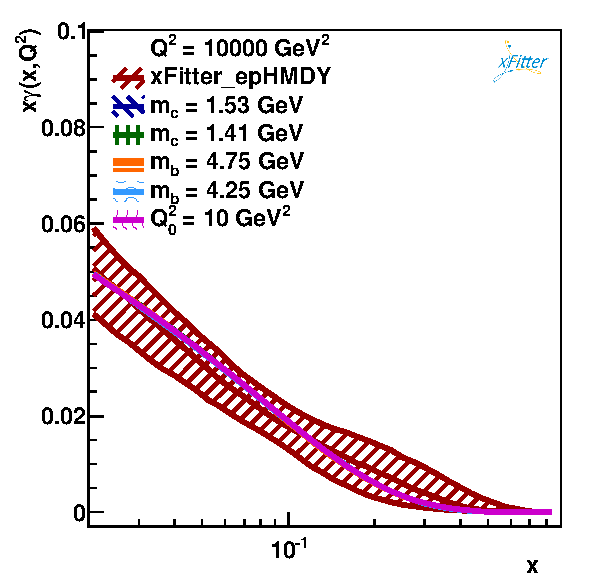
\includegraphics[width=8cm]{figs/q2_10000_pdf_ph_model_2}
\caption{Comparison between the baseline determination of
  $x\gamma(x,Q^2)$ at $Q^2=10^4$ GeV$^2$ in the present
  analysis with the central value of those  fits for which one input parameter has been varied.
  %
 The following variations have been considered: $r_s$, $Q^2_{\rm cut}$, $\alpha_s$ (left plot) and
$m_c$, $m_b$, $Q_0^2$ (right plot), see text for more details.
  %                   
}
\label{fig:model}
\end{figure}
%%%%%%%%%%%%%%%%%%%%%%%%%%%%%%

Another important check of the robustness of the present determination of
$x\gamma$ can be obtained by comparing the baseline fit with further
fits where a number of new free parameters are allowed in the PDF
parametrization, in addition to those listed in Eq.~(\ref{eq:param}).
%
Fig.~\ref{fig:param} shows the impact of three representative
variations (others have been explored, leading to smaller
differences): more flexibility to the gluon distribution, allowing it
to become negative at the initial scale (labeled by ${\rm neg}$), adding on top $D_{u_v}$,
and then $D_{\bar{u}}+D_{\bar{d}}$.
%
As before, all variations are contained within the MC PDF uncertainty
bands, though the impact of the parametrization variations is larger
than that of the model variations: in the case of the
${\rm nefg}+D_{\bar{u}}+D_{\bar{d}}$ variations, the central value is
at the edge of the lower uncertainty band.
%
Importantly, once this additional uncertainty coming from the
parametrization variations is accounted for, the agreement of the present fit
with LUXqed and HKR16 improves in the region around $x\simeq 0.02$.

An important cross-check of the robustness of the estimated
uncertainty of the photon PDF in this analysis is provided by the
comparison of the Monte-Carlo method with the Hessian method.
%
In Fig.~\ref{fig:photon_mc_vs_hessian} we show this comparison, which
indicates a reasonable agreement between the two methods.
%
In particular, the central values of the photon obtained with the two
fitting techniques are quite similar to each other.

%%%%%%%%%%%%%%%%%%%%%%%%%%%%%%%%%%%
\begin{figure}[t]
\centering
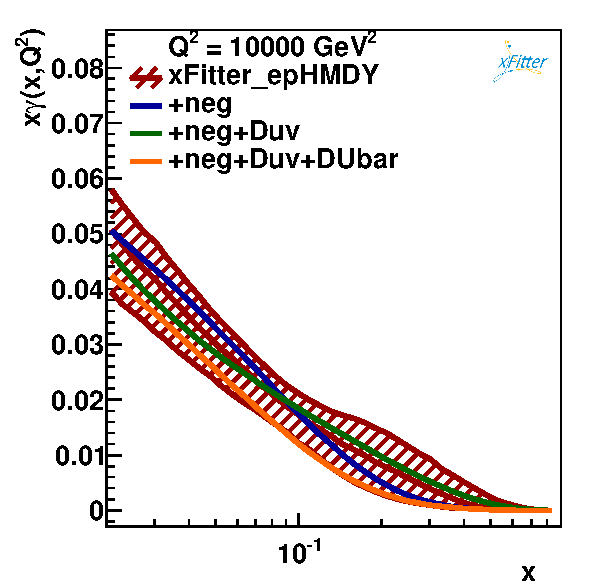
\includegraphics[width=8cm]{figs/q2_10000_pdf_ph_param_var.pdf}
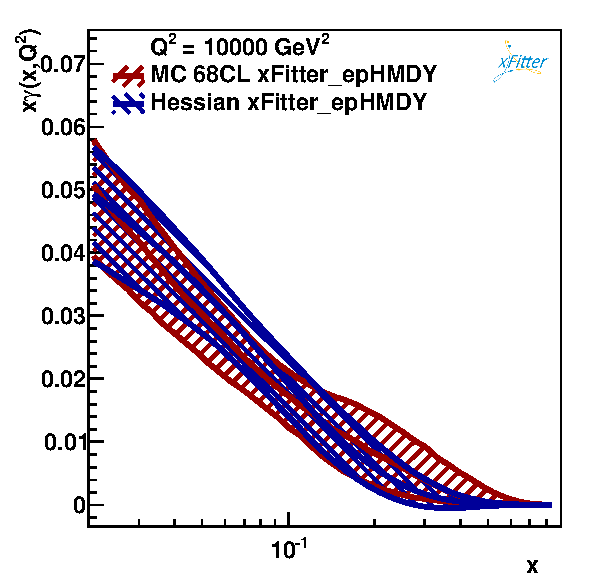
\includegraphics[width=8cm]{figs/photon_mc_vs_hessian} 
\caption{Left: the impact on $x\gamma(x,Q^2)$ at $Q^2=10^4$ GeV$^2$
  in fits where a number of additional free parameters are allowed
  in the PDF parametrization as compared to Eq.~(\ref{eq:param}).
  %
  In particular, the parametrization variations that have been explored
  are: more flexibility to the gluon distribution, allowing
  it to become negative
 (labeled by ${\rm neg}$), adding on top $D_{u_v}$, and then $D_{\bar{u}}+D_{\bar{d}}$.
 %
 Right: comparison between the fits of $x\gamma(x,Q^2)$ obtained with the
  Monte Carlo and the Hessian methods at $Q^2=10^4$ GeV$^2$.
  %
  In both cases, the PDF error band corresponds to the 68\% confidence
  level uncertainties.  }
\label{fig:param}
\label{fig:photon_mc_vs_hessian}
\end{figure}
%%%%%%%%%%%%%%%%%%%%%%%%%%

%\subsection{Perturbative stability of $x\gamma(x,Q^2)$}

An interesting exercise is to quantify the perturbative stability of
the present fit of the photon PDF $x\gamma(x,Q)$ with respect to the inclusion
of NNLO QCD corrections in the analysis.
%
To study this, Fig.~\ref{fig:nlo_vs_nnlo} shows a
comparison between the baseline fit of $x\gamma(x,Q)$, based on NNLO
QCD + NLO QED theory, with the central value resulting from a fit
based instead on NLO QCD theory (with the QED part identical in both
cases).
%
For the NNLO fit, only the experimental PDF uncertainties, estimated
using the Monte-Carlo method, are shown.

From the comparison of Fig.~\ref{fig:nlo_vs_nnlo}, it is clear that the
fit of $x\gamma(x,Q)$ exhibits a reasonable perturbative stability,
since the central value of the NLO fit is always contained in the
one-sigma PDF uncertainty band of the baseline determination based on
NNLO QCD + NLO QED.
%
The agreement between the two fits is particularly good for
$x\gsim 0.1$, where the two central values are very close to each
other.

%%%%%%%%%%%%%%%%%%%%%%%%%%%%%%%%%%%%%%%%%%%%%%%%%%%%%%%%
\begin{figure}[t]
\centering
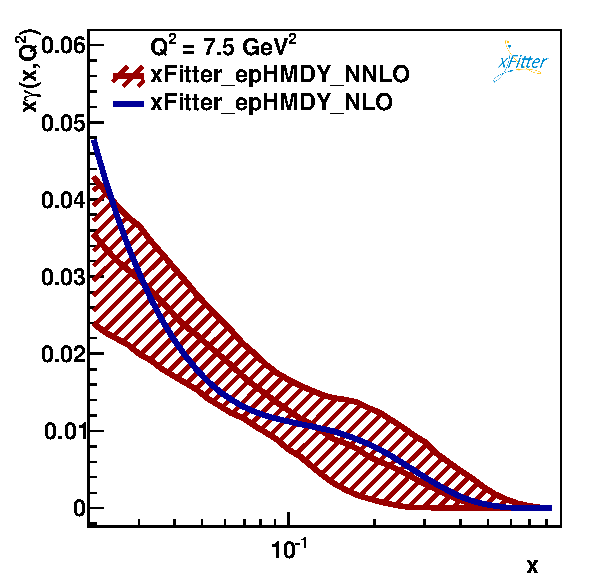
\includegraphics[width=8cm]{figs/q2_7_5_pdf_ph_NLOvsNNLO.pdf}
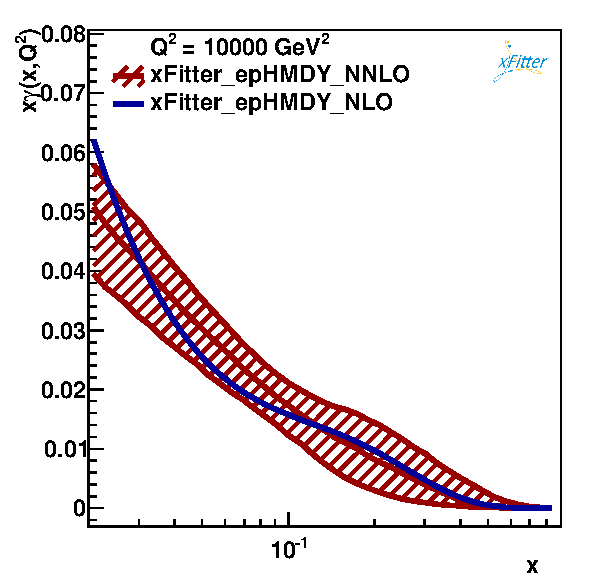
\includegraphics[width=8cm]{figs/q2_10000_pdf_ph_NLOvsNNLO.pdf}
\caption{Left: comparison between the baseline
  fit of $x\gamma(x,Q^2)$ (NNLO QCD + NLO QED) with the central value
  resulting from a NLO QCD+QED fit, at $Q^2=7.5$ GeV$^2$.
  %
  In the former case, only the experimental (Monte Carlo) PDF
  uncertainties are shown.
  %
  Right: same comparison but at evolved scale of $Q^2=10^4$ GeV$^2$.  }
\label{fig:nlo_vs_nnlo}
\end{figure}
%%%%%%%%%%%%%%%%%%%%%%%%%%%%%%%%%%%
